\section{Logistic Regression}
\smallskip \hrule height 2pt \smallskip

Another probabilistic approach to classification (categorical predictions).   \hfill \\
Can use discrete or continuous outputs. \hfill \\ % https://www.youtube.com/watch?v=zAULhNrnuL4
\hfill \\ 

\underline{Summary from non-class sources:} \hfill \\
% https://www.youtube.com/watch?v=-Z2a_mzl9LM
We are still using linear regression in the inputs, but putting the result into a sigmoid function. \hfill \\
Recall $w_0 + w_1 x_1 + w_2 x_2 + w_3 x_3 = w^Tx$ and $x = (1, x_1, x_2, x_3)$.  \hfill \\
$P(death|x) = \sigma(w^Tx)$  %https://www.youtube.com/watch?v=-Z2a_mzl9LM
where $\sigma$, the sigmoid function,  converts your regression output into a sigmoid curve. \hfill \\
$\displaystyle \sigma(a) = \frac{1}{1+ e^{-a}} = \frac{1}{1+ e^{-(w_0 + w_1 x_1 + w_2 x_2 + w_3 x_3)}} = \frac{1}{1+ e^{-(w^Tx)}}$   \hfill \\ % https://www.youtube.com/watch?v=-Z2a_mzl9LM
\hfill \\

% https://www.youtube.com/watch?v=_Po-xZJflPM  :
We can convert this to a linear relationship by "taking the logit". \hfill \\
The logit (log odds) is the inverse of the logistic.  \hfill \\ %  https://en.wikipedia.org/wiki/Logistic_regression
$F(x) = \sigma(a)$ above.  It is the probability that the dependent variable equals a case, given some linear combination of the predictors.  It can range from $- \infty$ to $\infty$   % https://en.wikipedia.org/wiki/Logistic_regression
The logit is $\ln \frac{F(x)}{1-F(x)}$, or equivalently, after exponentiating both sides: \hfill \\
$\frac{F(x)}{1-F(x)} = e^{w^Tx}$  \hfill \\
The logit (i.e., log-odds or natural logarithm of the odds) is equivalent to the linear regression expression.

 


Note used odds ratio: $\frac{p}{1-p}$  \hfill \\
$\logit(\frac{1}{1+ e^{-(w^Tx)}}) = \log(\frac{\frac{1}{1+ e^{-(w^Tx)}}}{1-\frac{1}{1+ e^{-(w^Tx)}}}) $  \hfill \\ % https://www.youtube.com/watch?v=_Po-xZJflPM
We can now proceed with linear regression.  \hfill \\
Note that our predictions are now on the log scale; this impacts interpretation of the coefficients.  \hfill \\  %https://www.youtube.com/watch?v=_Po-xZJflPM 

\hfill \\ \hfill \\   

\underline{Lecture's presentation:} \hfill \\

Notation:  \hfill \\
\begin{itemize}
	\item $y^j$: the $j^{th}$ class  %(?)
	\item $x^j$: the $j^{th}$ training example
\end{itemize}

Once again we don't want to try to estimate $P(X,Y)$; that is challenging due to the size of the distribution. \hfill \\
We could make the Naive Bayes assumption and only need to calculate $P(X_i | Y)$, 
but if we want $P(Y|X)$, why not learn that directly?  You can use logistic regression. 
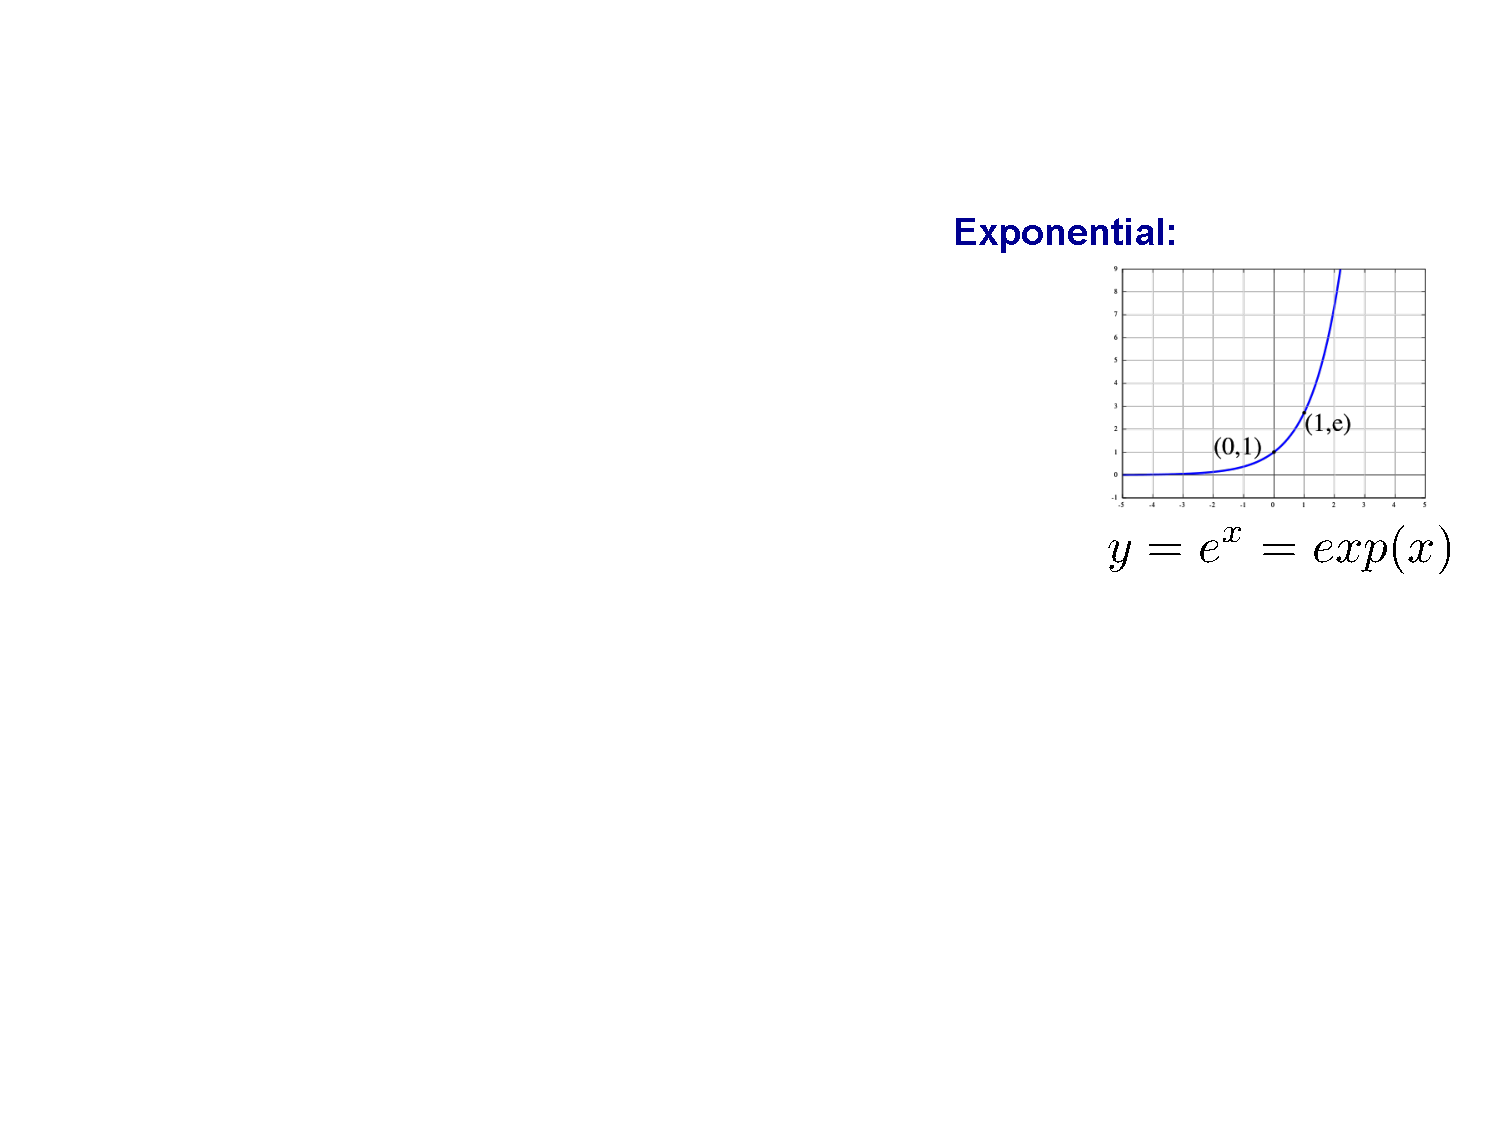
\includegraphics[width=1.5in]{figures/expo.pdf}     \hfill \\
\hfill \\

Reuse ideas from regression, but let the y-intercept define the probability.  \hfill \\
$P(Y=1|\bm{X, w}) \propto exp(w_0 + \sum_i w_i X_i)$  \hfill \\
With normalization constants:  \hfill \\
$\displaystyle  P(Y=0|\bm{X, w}) \frac{1}{1+ exp(w_0 + \sum_i w_i X_i)} $ \hfill \\
$\displaystyle  P(Y=1|\bm{X, w}) \frac{exp(w_0 + \sum_i w_i X_i)}{1+ exp(w_0 + \sum_i w_i X_i)} $ \hfill \\
Logistic function: 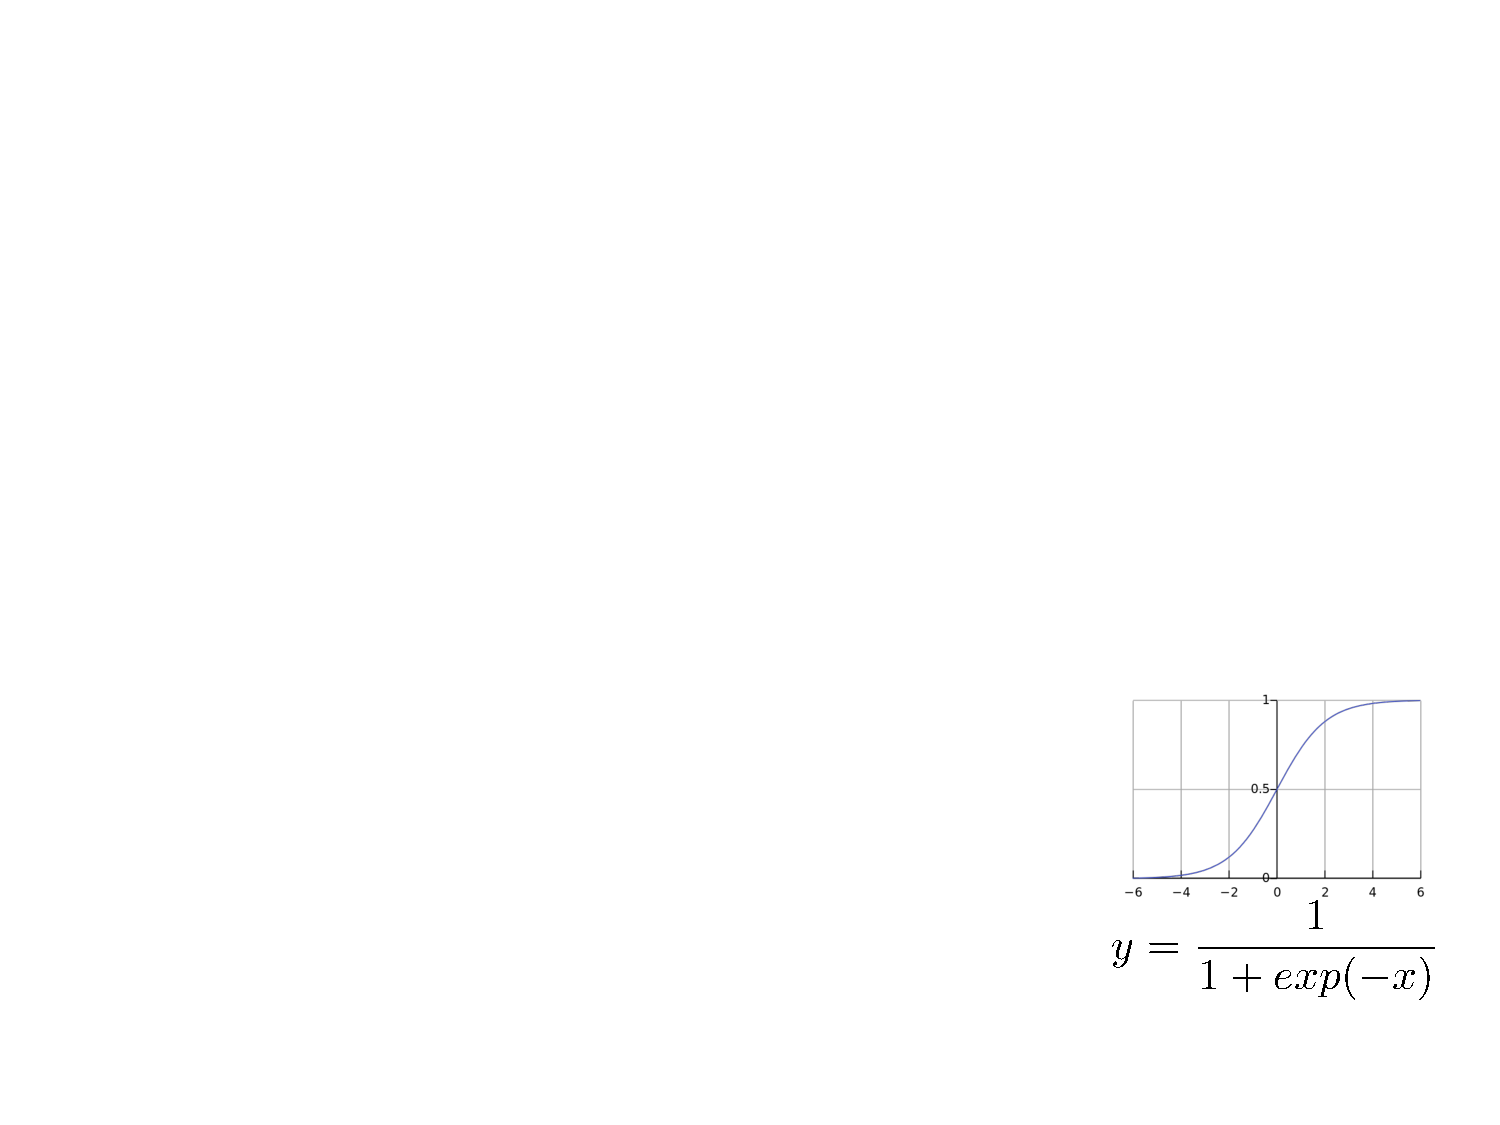
\includegraphics[width=1in]{figures/logistic.pdf}     \hfill \\
 \hfill \\
 
Making a decision boundary out of logistic equations:  \hfill \\
Output the $Y$ with the highest $P(Y|X)$.   \hfill \\
If binary Y, output Y=1 if $\displaystyle 1 < \frac{P(Y=1|X)}{P(Y=0|X)}$  \hfill \\
That simplifies to just $1 <exp(w_0 + \sum_i w_i X_i)$ or \hfill \\
$0 <w_0 + \sum_i w_i X_i$   \hfill \\
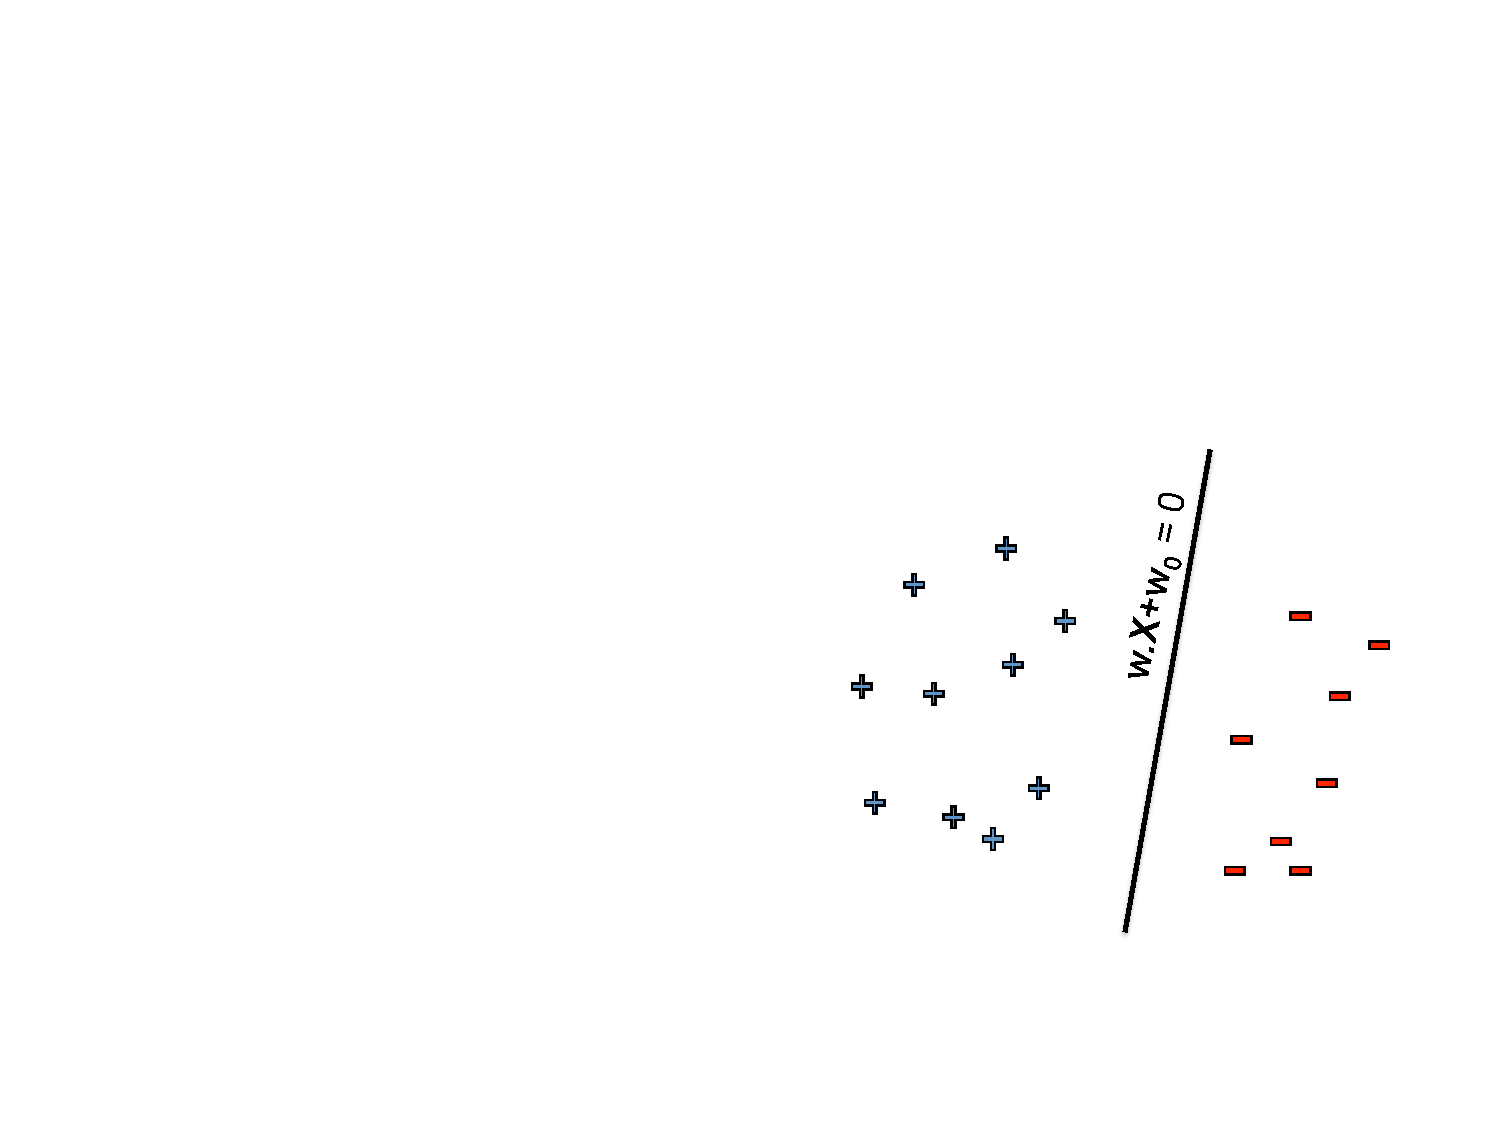
\includegraphics[width=.8in]{figures/logistic_boundary_linear.pdf}     \hfill \\
\textbf{The decision boundary is a line (or hyperplane), hence we have a linear classifier!} \hfill \\  \hfill \\

For $ \displaystyle P(Y=0 | \bm{X,w}) = \frac{1}{1 + exp(w_o + w_1 x_1)}$:  \hfill \\
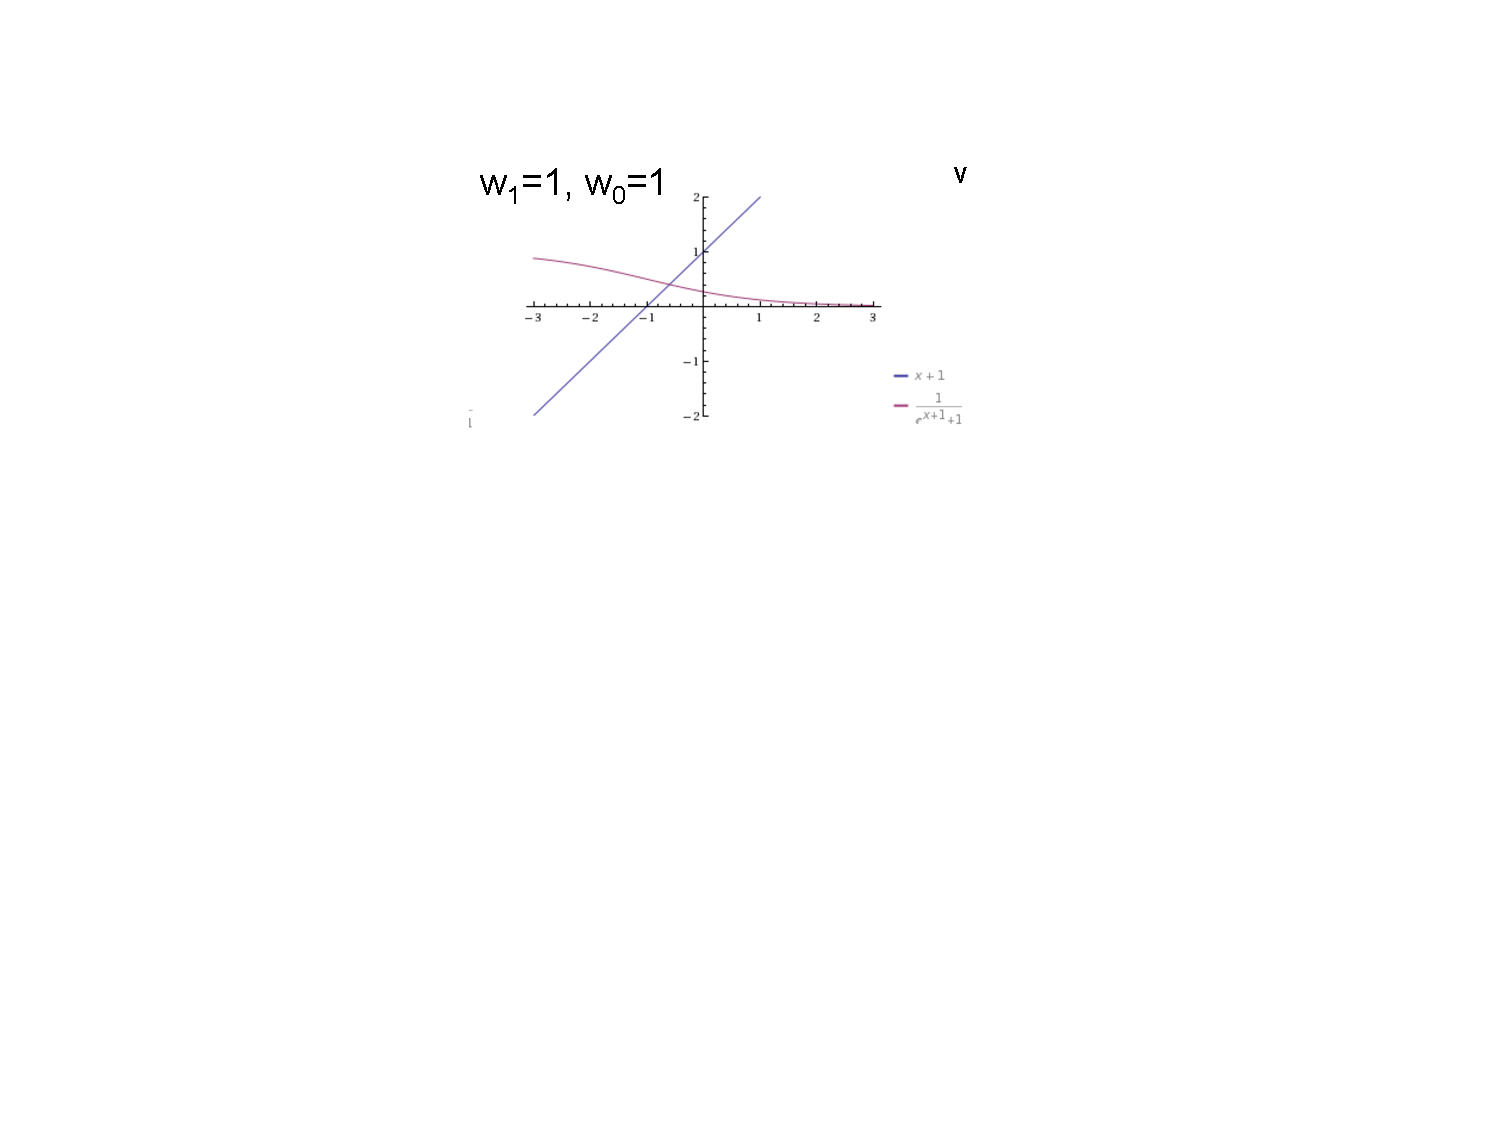
\includegraphics[width=2in]{figures/decision_boundary_example.pdf}   \hfill \\
(See notes for more $w_0, w_1$ values plotted.)  \hfill \\
In these plots, Y is the probability that the class is 1.    \hfill \\
The red curve is the sigmoid.  The blue line is the decision boundary.  \hfill \\
The decision boundary is from the equation $0 = w_1X + w_0$.  \hfill \\
% Erick advice: ignore the blue lines entirely.  don't need them to find probability distribution. 

\hfill \\
Larger weights result in a sharper curve.  The bias $w_0$ shifts there the middle of the curve is.   \hfill \\
The red sigmoid defines a probability distribution over $Y$ in \{0,1\} for every possible input X. \hfill \\
\hfill \\
The decision boundary leads to $P(Y=0|X, w) = 0.5$ when you are at the $y=0$ point on the line.   \hfill \\
(E/J words:  when the blue line crosses the x axis, that's when the sigmoid curve is above 1/2, which corresponds to classifying it as a no/0.)  \hfill \\
The slope of the line defines how quickly the probabilities go to 0 or 1 around the decision boundary. 
\hfill \\

2D inputs: \hfill \\
For $ \displaystyle P(Y=0 | \bm{X,w}) = \frac{1}{1 + exp(w_o + w_1 x_1 + w_2 x_2)}$:  \hfill \\
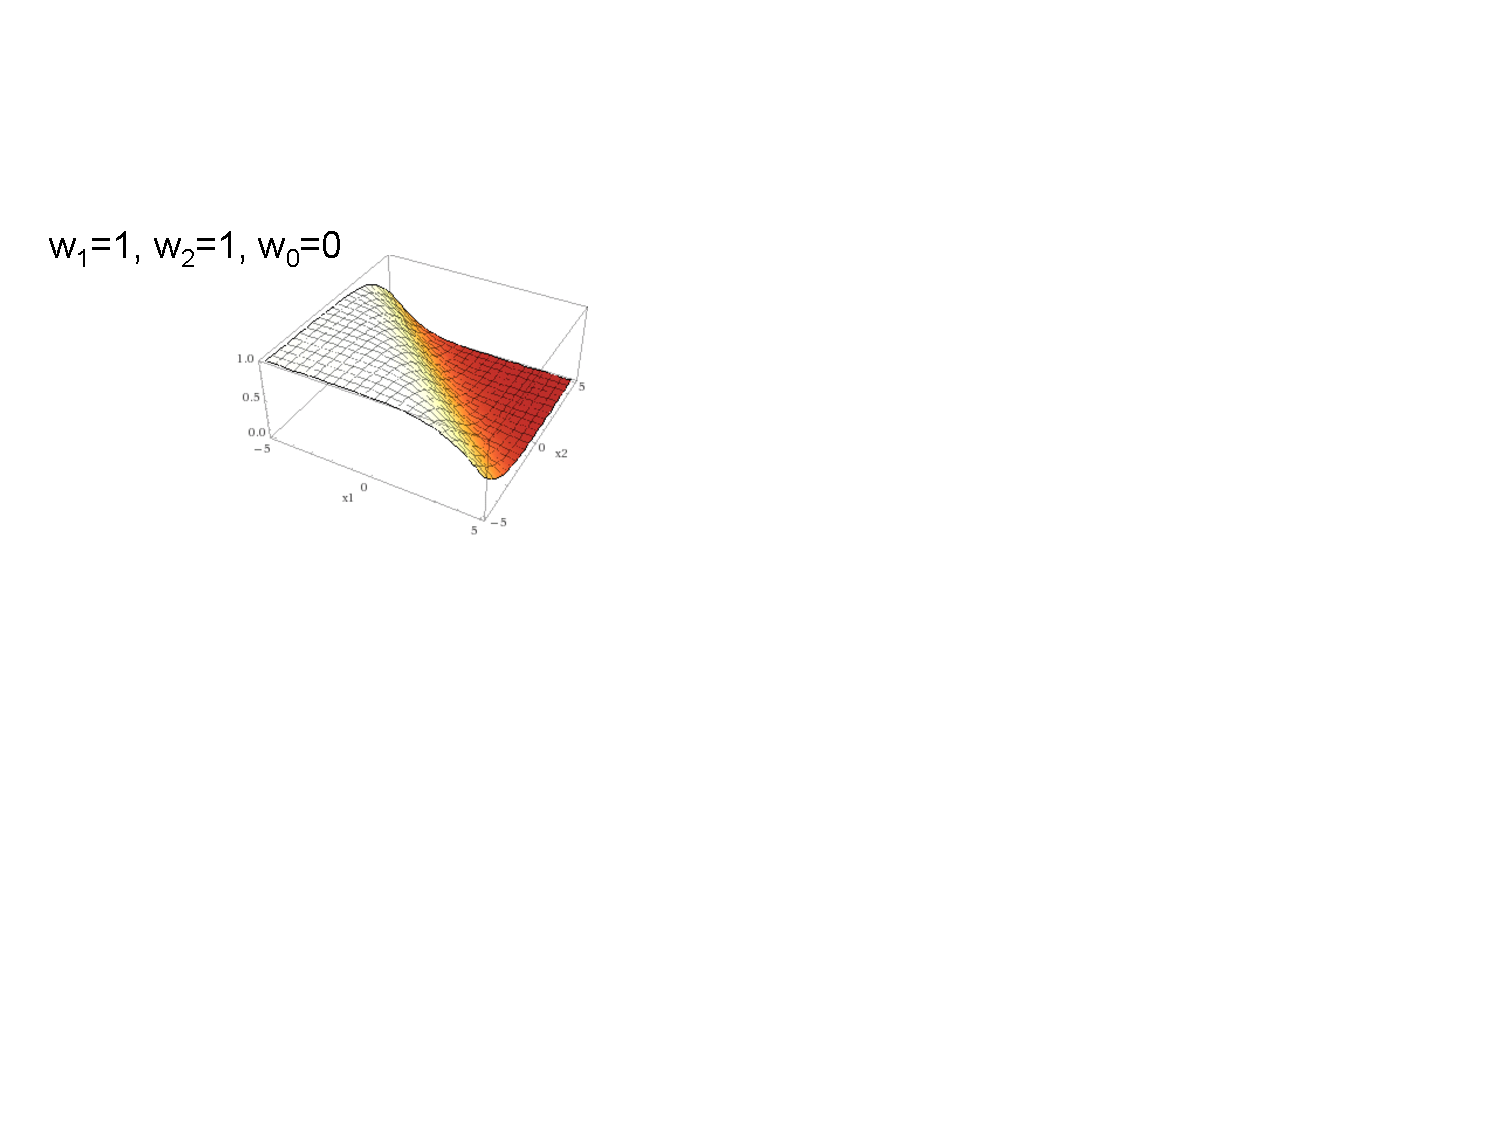
\includegraphics[width=2in]{figures/decision_boundary_example-2D.pdf}   \hfill \\

$P(Y=0 | X, w)$ decreases as $w_0 + \sum_i w_i x_i$ increases. 
Again, if you set the stuff inside the exponential to zero, you get the decision boundary hyperplane.

\subsubsection{Finding the w coefficients}
Generative (Naive Bayes) loss function: 
Now $j$ is a data point with observations indexed over $i$.


\begin{align*}
	\ln P(D | \bm{w}) = \sum_{j=1}^N  &  \ln P(x^j, y^j | \bm{w}) \mbox{   } \mbox{    (the full log-likelihood)}\\
					& \mbox{use Bayes' rule to rewrite conditionally}  \\  % J added this line. 
					= \sum_{j=1}^N  &  \ln [P(y^j | x^j, \bm{w}) P(x^j | \bm{w})] \\ % J added this line. 
				=  \sum_{j=1}^N  & \ln P(y^j | x^j , \bm{w}) + \sum_{j=1}^N \ln P(x^j | \bm{w})
\end{align*}

We decide to ignore the 2nd term because it won't help you get better predictions for that data anyway. 
Or, "From a machine learning perspective, "God gave us the data" and we don't care about the 2nd sum."  % Erick 2/6/2016

Professor Farhadi is calling this first time a discriminative (logistic regression) loss function:  \hfill \\
It is helping you discriminate between different classes.  It's not going to help you model the data. 
This is unlike regression; we don't care about the value it puts out.  We only care about what the resulting class is.  \hfill \\

% Erick. 
This is the difference between statistics and machine learning.  We only care about getting the best $\bm{w}$ for discriminating between classes. 

\textbf{Conditional Data Likelihood:} 
"Conditional" because you are conditioning on what $\bm{X}$ is. 
\begin{align*}
	\ln P(D_Y | D_{\bm{X}}, \bm{w}) = \sum_{j=1}^N \ln P(y^j | \bm{x}^j, \bm{w})
\end{align*}
$D_Y$ = ???  \hfill \\
$D_{\bm{X}}$ = ???   \hfill \\
Doesn't waste effort learning $P(X)$.  Focuses on $P(Y| \bf{X})$, which is all that matters for classification. \hfill \\
Discriminative models cann't compute $P(\bm{x}^j | \bm{w})$!  ??? 
\hfill \\

\subsubsection{Conditional Log Likelihood}
(the binary case only).  \hfill \\
$P(Y=0 | \bm{X}, \bm{w}) = \frac{1}{1 + \exp(w_0 + \sum_i w_i X_i)}$  \hfill \\
$P(Y=1 | \bm{X}, \bm{w}) = \frac{\exp(w_0 + \sum_i w_i X_i)}{1 + \exp(w_0 + \sum_i w_i X_i)}$  \hfill \\

($ l( \bm{w} )$ is conditional data log-likelihood.)  
\begin{align*}
	l( \bm{w})  \equiv  &  \sum_j \ln P(y^j | x^j, \bm{w})  \\
	& \mbox{Since $y^j$ is in \{0, 1\}, sum over the two cases: }   \\
	& \mbox{(the $y^j$ and $(1-y^j)$ act like delta functions)}   \\
	l(\bm{w})  =  & \sum_j y^j \ln P(y^j = 1 | x^j, \bm{w}) +(1 - y^j) \ln P(y^j = 0 | x^j, \bm{w})  \\
	& \mbox{plug in the definition of the likelihoods and do algebra to get:}  \\
	=& \sum_j  y^j (w_0 + \sum_i^n w_i x_i^j)  - \ln(1 + \exp(w_0 + \sum_i^n w_i x_i^j)) 
\end{align*}	

While we can't find a closed-form solution to optimize $l(\bm{w})$,  $l(\bm{w})$ is concave so we can to gradient \underline{as}cent. 

\subsubsection{Gradent ascent to optimize w}
Conditional likelihood for Logistic Regression is convex.  (see above)  \hfill \\
\textbf{Gradient}:  \hfill \\
\begin{align*}
	\nabla_w l(\bm{w}) = [\frac{\partial l(\bm{w})}{\partial w_0}, \dots, \frac{\partial l(\bm{w})}{\partial w_n}]'  \hfill \\
\end{align*}
	(The $'$ at the end is for transpose b/c usually a column vector.)  \hfill \\
\textbf{Update Rule:} \hfill \\
\begin{align*}
	\Delta \bm{w} &= \eta \nabla_{\bm{w}} l(\bm{w})
\end{align*}
$\eta$ is the learning rate.  $\eta > 0$.

Your next weights $(t+1)$ become: 
$w_i^{(t+1)} \leftarrow w_i^{(t)} + \eta \frac{\partial l(\bm{w})}{\partial w_i}$   \hfill \\
\hfill \\
Gradient ascent is the simplest  of optimization approaches.  Note that conjugate gradient ascent is much better (see reading).(?)

Vocab \hfill \\
\begin{itemize}
	\item \textbf{discriminative}:  estimates joint probabilities.  E.g. $p(Data, Zebra)$, $p(Data, No Zebra)$. 
	\item \textbf{generative}:  E.g. $p(Zebra | Data)$, $p(No Zebra | Data)$. 
\end{itemize}



Andrew Ng: \hfill \\
* gives numbers between 0 and 1 (good for classification)   \hfill \\
* called "logistic regression" but it is really for classification.  (don't be confused by "regression") \hfill \\
* "sigmoid function" and "logistic function" are essentially synonomous.  \hfill \\
 
